\documentclass[a4paper]{article}

\usepackage[english,francais]{babel}
\usepackage[utf8]{inputenc}
\usepackage{amsmath}
\usepackage{graphicx}
\usepackage[colorinlistoftodos]{todonotes}
\usepackage{float}


\author{Florian Toqué}

\date{20 Octobre, 2015}


\title{Calcul de représentation d'images et apprentissage supervisé\\}


\begin{document}

\maketitle



\selectlanguage{francais}
\begin{abstract}


Ce rapport porte sur un travail effectué au cours de l'UE RDFIA du Master informatique spécialité Imagerie de l'université Pierre et Marie Curie (Paris). Le travail réalisé consiste à mettre en place un système de classification d’images par apprentissage supervisé. Une fois appris ce système de classification est en mesure d’affecter une des 15 catégories sémantiques à une image de test donnée. Dans ce rapport nous expliquons une des parties nécessaires à ce système qui est la représentation d'image en Bag of Words et l'apprentissage supervisé (SVM). 
\end{abstract}
\newpage
\section{Introduction}
Lors de ce projet nous avons implémenté deux parties, le calcul des BoW qui représentent les images et la formation d'un classifieur multi-classe (SVM en un contre tous).


\section{Calcul de représentation d'image: le modèle Bag of Words (BoW)}
Afin de classifier des images il est tout d'abord nécessaire de les représenter de manière uniforme. La technique employée ici est de représenter chaque image sous forme de Bag of Words. Chaque image est en premier lieu représentée par un ensemble de SIFTS  calculés au préalable, nous avons aussi calculé à l'aide d'un algorithme de clustering, un dictionnaire contenant les mots visuels les plus représentatifs de l'ensemble des images que nous avons à notre disposition. On représentera alors une image sous forme de vecteur (histogramme contenant l'importance de chaque mot visuel sous forme de scalaire pour définir l'image). 
\subsection{Visualisation du dictionnaire visuel}
Le dictionnaire visuel contient l'ensemble des "mots visuels" (1000) les plus représentatifs de l'ensemble de la base 15-scenes, calculé dans un travail précédent à l'aide de l'algorithme du KMeans. Voici sa visualisation:\\
\begin{center}
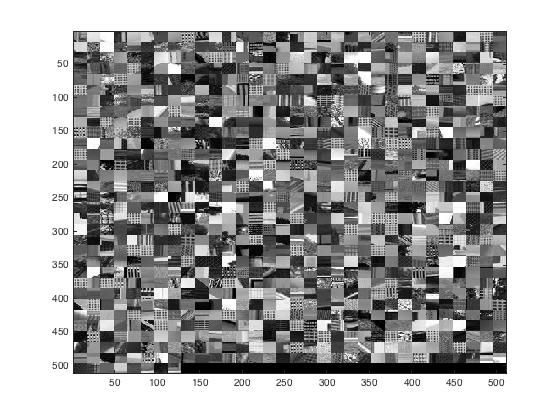
\includegraphics[scale=0.5]{dico}
\end{center}
\subsection{Calcul de BoW sur des images et visualisation des résultats}
Nous voulons représenter les images d'une manière uniforme pour pouvoir les classifier.\\
Pour ce faire deux étapes sont nécessaires, la première est le cooding, cette étape consiste à calculé pour chaque SIFT de l'image le mot du dictionnaire le plus similaire. Une fois cette étape effectuée il suffit de faire l'aggrégation (pooling) du nombre de mots trouvés pour chaque SIFTS et de diviser l'ensemble par le nombre de SIFTS de l'images. Nous obtenons alors la représentation d'une image sous forme de vecteur (BOW) de la taille du dictionnaire contenant à l'emplacement de chaque mot visuel son importance pour la représentation de l'image sous forme de scalaire.
\\
Voici la visualisation de l'histogramme d'une image, le mot 780 à 4,5\% dans l'image, le mot 70, 2\%:\\
\begin{center}
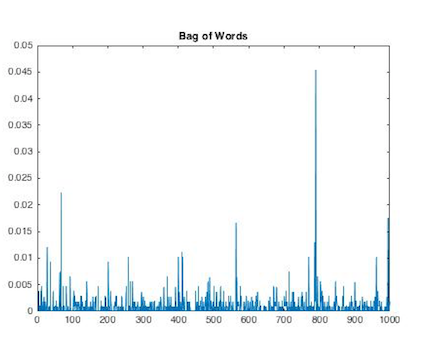
\includegraphics[scale=0.5]{bowHisto}
\end{center}

Voici la visualisation d'une image, de ses 8 mots les plus fréquents ainsi que leurs localisations:\\
\begin{center}
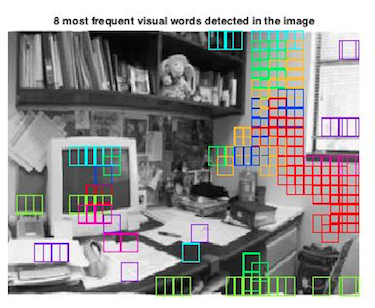
\includegraphics[scale=0.5]{bowLoc}
\end{center}
\subsection{Calcul de l’ensemble des BoW sur la base}
Afin de classifier les 4485 images de la bases nous devons calculer leurs BoW. Pour ce faire nous faisons comme précédemment pour toutes les images de la base en stockant leurs BoW dans un fichier.



\section{Apprentissage supervisé pour la classification sémantique d'images}
Chaque image est représentée sous forme d'un BoW qui est un vecteur de taille 1000. Pour classifier chaque image parmis les 15 catégories possible nous avons utiliser l'algorithme d'apprentissage SVM. Nous allons tout d'abord présenter cet algorithme de classification pour des données binaires, puis nous expliquerons comment il est utilisé pour classifier des données multi-classes.
\subsection{Apprentissage des SVM binaires}
Un classifieur SVM(support vector machines) est un algorithme d'apprentissage linéaire. Il permet de créer une frontière entre deux classes différentes tout comme un algorithme de régression logistique. L'avantage est qu'en plus de séparer l'espace binaire en deux espaces distincts, il maximise la marge qui existe entre l'hyperplan séparateur est les données ce qui revient en fait à résoudre un problème d'optimisation sous contrainte.

Voici la visualisation de la séparatrice d'un svm pour des données binaires:\\
\begin{center}
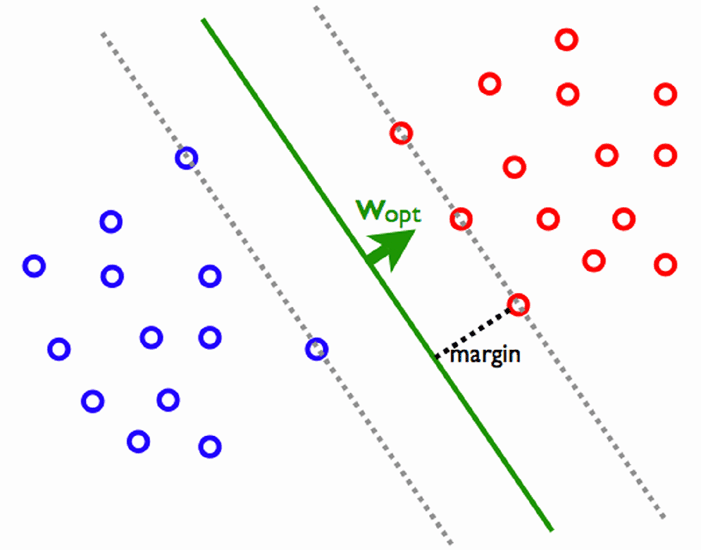
\includegraphics[scale=0.3]{svm}
\end{center}
\subsection{Formation d'un classifieur multi-classe}
Notre problème de classification d'image n'est pas une classification binaire, en effet nous devons catégoriser nos images parmi 15 classes différentes et non deux. Pour ce faire nous allons créer 15 classifieurs binaires chacun correspondant à une classe versus toutes les autres. Pour classifier une image nous classifierons l'image avec les 15 classifieurs et choisirons la classe dont le score sera maximal.
\newpage
Voici la visualisation de la matrice de confusion obtenue après la catégorisation de notre ensemble de test:\\
\begin{center}
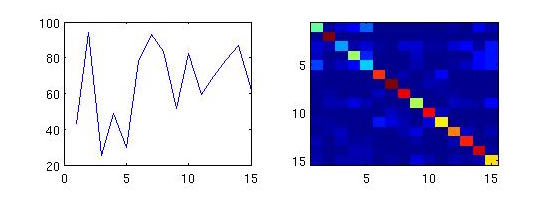
\includegraphics[scale=0.7]{confusion}
\end{center}
Nous remarquons que les images des catégories 3 et 5 n'ont pas été très bien catégorisés (30\% de bonne classification)
\subsection{Carte de chaleur de classification}
Afin d'analyser l'impact de chaque descripteur local lors de la classification d'image, nous avons mis en place une fonction permettant de calculer une "carte de chaleur de classification".  Nous avons donc calculé pour chaque descripteur local sa contribution lors de la classification à l'aide de la formule suivante:  $\frac{1}{N}  w_m^*$ \\\\
\textbf{Question: Montrer que la contribution de chaque descripteur $x_j$ dans la fonction de classification s'écrit $p(x_j) = \frac{1}{N}  w_m^*$} ?\\\\
On a:\\
\begin{align*}
\nonumber {}f\left ( b \right )&= <w,b > \\
\nonumber {}&= \sum_{m=0}^{N}w_m.b_m\\
\nonumber {}&=\sum_{m=1}^{N}w_m.\frac{1}{N}\sum_{i}\alpha_{i,m}\\
\nonumber {}&=\frac{1}{N}\; \sum_{i=1}^{N}\sum_{m=0}^{N}\alpha_{i,m}.w_m\\
\nonumber {}&=\sum_{i=1}^{N}\sum_{m=1}^{n}\frac{\alpha_{i,m}}{N}w_m
\end{align*}
or \\
\begin{align*}
\sum_{m=1}^{n}\frac{\alpha_{i,m}}{N}w_m &= \sum_{i=1}^{N}\frac{1}{N}w_{m^*}
\end{align*}

Ceci est plus une explication qu'une démonstration..\\
N correspond au nombre de descripteurs locaux dans l'image et $m^*$ au mot visuel le plus proche de la classe k en question. Il suffit alors de regarder quel est le poids associé à ce mot visuel dans le modèle de classification de la classe k pour connaitre sa contribution. Etant donné qu'il s'agit d'une probabilité il faut divisé ce poids par le nombre de descripteurs locaux. Nous obtenons ainsi pour chaque descripteur local un scalaire représentant son importance pour la catégorisation avec une certaine probabilité. Ceci nous permet de faire cette visualisation qui représente pour chaque descripteur, l'importance qu'il a dans la catégorisation. \\
Visualisation de la HeatMap:\\

\begin{center}
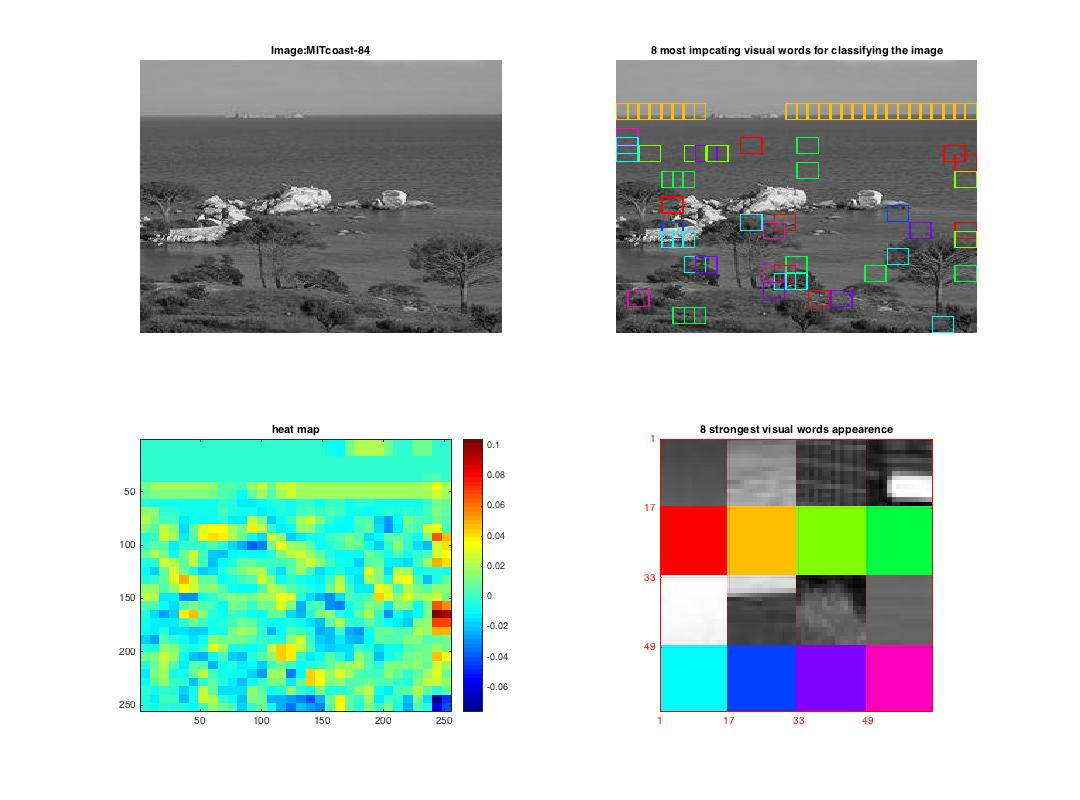
\includegraphics[scale=0.3]{heatMap}
\end{center}
On remarque bien que les sifts se situant dans l'image entre la mer et le ciel ont un poids fort dans la classification de cette image grâce à la carte de chaleur de classification. (image en bas à gauche)\\



\section{Bonus: analyse de résultats et limitations de la représentation utilisée}
\subsection{Prise en compte de l'information spatiale dans la représentation BoW}
Dans le travail présenté jusqu'ici nous avons utilisé les BoW sans information spatiale, c'est à dire que la même image dupliquée d'une manière identique Image1 et dupliquée avec une rotation de manière inversée Image2 sera considérée comme la même image alors que nous ne voulons pas forcément qu'une telle similarité apparaisse. Pour cela l'article [3] "Linear spatial pyramid matching using sparse coding for image classification" préconise de créer plusieurs niveaux de représentations de BoW augmentant l'importance de l'information spatiale au fur et à mesure que l'information est codée dans les "étages" supérieurs de la pyramide. Il faut alors pondérer l'importance de chaque niveau de la pyramide en fonction de l'importance que nous voulons au niveau spatiale.\\
Etant donné que notre score est de 66\% de bonne classification sur l'ensemble de test, les résultats obtenus à l'aide de l'algorithme scSPM (80\%) sont bien meilleurs.
\subsection{Différences dans les méthodes de coding/pooling pour la formation des BoW}
Différentes méthode de coding et pooling sont présentés dans l'article 1 "Learning mid-level features for recognition" Y.Boureau,Y.LeCun. La méthode de cooding décrite consiste à concaténer l'information des SIFTs se situant dans un voisinage proche, dans le but de garder une information de spatialisation. Le pooling est la manière de calculer l'importance de chaque sifts pour la représentation d'une image. La méthode obtenant les meilleurs résultats est celle du max-pooling ce qui est due à la robustesse par rapport aux variations spatiales.


\subsection{Normalisation des BoW ($l_1$ vs  $l_2$)}
La normalisation $L_1$ du BOW consiste à assigné un unique mot visuel à chaque SIFT de l'image, cette normalisation pouvant être trop restrictive la normalisation $L_2$ a été testé dans l'article "Linear spatial pyramid matching using sparse coding for image classification" J.Yang. La normalisation $L_2$ ayant moins de contrainte elle garde plus d'information et est donc plus robuste pour le coding.
\subsection{Différences entre Bow et descripteurs obtenus à partir de CNN}
La différence majeure est que le fait d'apprendre sur une plus grosse base de donnée permette aux CNN de ressortir plus d'information et donc de mieux catégoriser. En catégorisant à l'aide des BOW cette astuce ne permet pas d'obtenir de meilleurs résultats puisque l'on ne ressort pas plus d'information.
\section{Conclusion}
Nous avons classifier des images en les représentant sous forme de BOW, plusieurs méthodes permettent d'obtenir de meilleurs résultats comme différentes méthode de cooding/pooling, utilisation de la normalisation et de l'information spatiale à prendre en compte. Malgré de bons résultats obtenus à l'aide de ces BOW les meilleures performances sont obtenues à l'aide des descripteurs venant des CNN de part la plus grande quantité d'information que ceux ci contiennent.
\end{document}